\section{Signal modelling}
\label{sec:signal_model}

The shape of the signal and background \myy distributions is described with analytical functions. Like in the past analysis \cite{Hasib:2238687}, the shape of \myy invariant mass distribution for signal events in each category is modelled with a \emph{double-sided Crystal Ball} (DSCB) function. It is a composite function with 6 parameters formed by a Gaussian core, which models the peak, and two power-law tails, as detailed in \Eqn{\ref{eq:DSCB}}:
\begin{align}
	f_\text{DSCB}(\myy) = N \times
	\begin{cases}
		e^{-t^{2}/2} & \text{if } -\alpha_{low} \leq t \leq \alpha_{high} \\
		\frac{ e^{-{}^{1}_{2} \alpha_{low}^{2}} } { \left[ \frac{1}{R_{low}} \left(R_{low} - \alpha_{low} - t \right) \right]^{n_{low}} } & \text{if } t < -\alpha_{low} \\
		\frac{ e^{-{}^{1}_{2} \alpha_{high}^{2}} } { \left[ \frac{1}{R_{high}} \left(R_{high} - \alpha_{high} + t \right) \right]^{n_{high}} } & \text{if } t > \alpha_{high} \\
	\end{cases}
	\label{eq:DSCB}
\end{align}
where $N$ is a normalization factor and the six parameters are
\begin{itemize}
	\item $\mu_\text{CB}$ and $\sigma_\text{CB}$ describe the mean and the width of the Gaussian core, which are combined in $t = \left(\myy - \mu_\text{CB}\right) / \sigma_\text{CB}$;
	\item $\alpha_{low}$ and $\alpha_{high}$ are the positions of the transitions with respect to $\mu_\text{CB}$ from the Gaussian core to power-law tails, in unit of $\sigma_\text{CB}$, on the low and high mass sides respectively;
	\item $n_{low}$ and $n_{high}$ are the exponents of the low and high mass tails. With the $\alpha$'s, they define $R_{low} = \frac{n_{low}}{\alpha_{low}}$ and $R_{high}$ similarly.
\end{itemize}

In the previous analysis \cite{Hasib:2238687}, the DSCB has showed a good $\chi^2$ in the signal only fit and gives a slightly smaller bias on the fitted signal yield using injection tests on Asimov background and signal MC. \\ The advantage of the DSCB is to well separate the contribution coming from the core and from the tails, making easier to apply systematic variations on the scale (on $\mu_\text{CB}$) and on the resolution (to $\sigma_\text{CB}$). \\

Thanks to the very precise knowledge of the Higgs mass from Run1 from the combination of ATLAS and CMS measurements ($\mH=125.09\err{0.21}\stat\err{0.11}\syst \, \si{\GeV}$)~\cite{HIGG-2014-14} and to the relatively small error of the mass scale systematics ($<1\%$), it is possible to parametrize the shape using just one set of MC samples simulated with the Higgs mass \mH fixed at \SI{125}{\GeV}. The MC sample combines all the production modes assuming Standard Model cross sections and the three MC types (mc16a+d+e) are weighted taking into account the relative luminosity of 2015/2016, 2017 and 2018 datasets, respectively. The generalization of the fitted model to any value of \mH (in a small interval close \SI{125}{\GeV}) is done with a simple shift of the $\mu_{CB}$ parameter ($\mu_\text{CB}= m_H + \mu_\text{CB}^{\SI{125}{\GeV}} - \SI{125}{\GeV}$).\\

\textcolor{red}{Systematic from mH:  Higgs mass: 125.09 +/- 0.24 GeV as photon energy scale (PES).}

The signal shapes are fitted in the fixed mass range \SIrange{105}{160}{\GeV} while leaving floating all the six parameters of the DSCB function. The signal models for each category are shown in \Fig{\ref{fig:signal_shapes}}. The same procedure is performed both for SM and BSM Monte Carlo samples, in every VBF categories, Optimal Observable bins and CP-mixing hypothesis the \myy models are determined by their best fit results from MC.

\begin{figure}[htbp]
  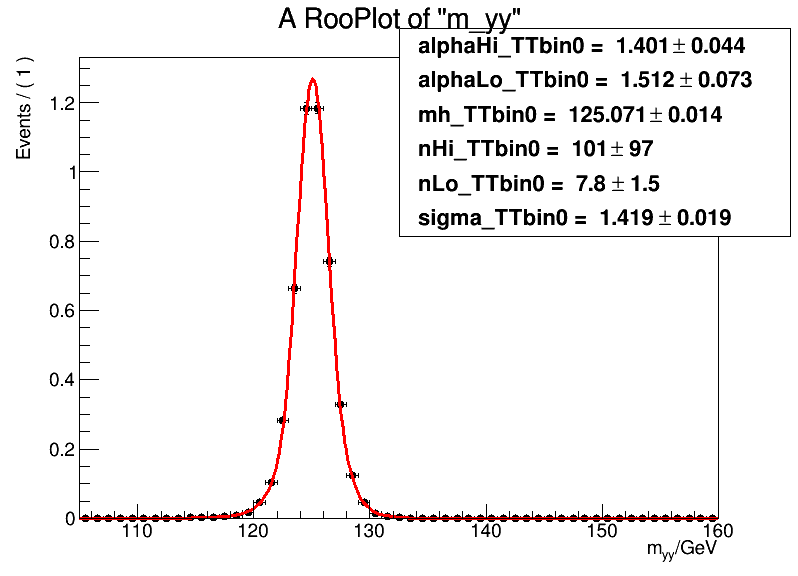
\includegraphics[width=.24\textwidth]{figure/sigmodel/SigFit_TTbin0.png}
  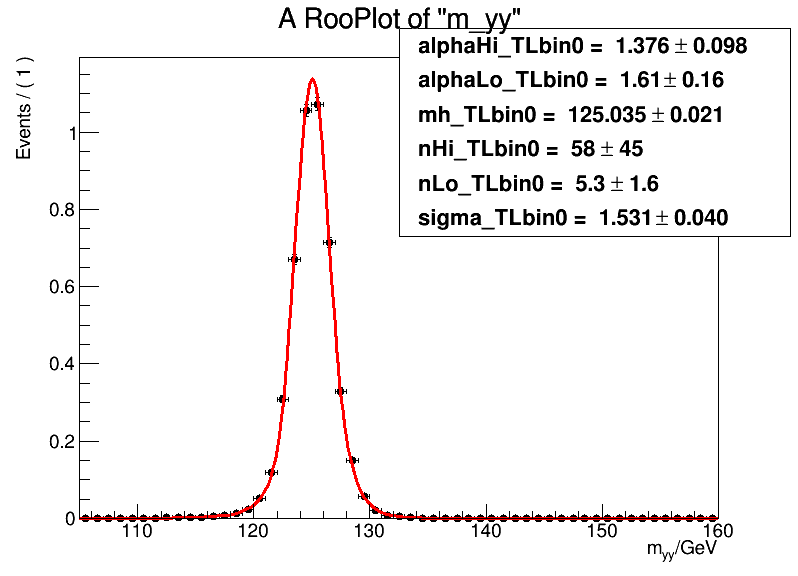
\includegraphics[width=.24\textwidth]{figure/sigmodel/SigFit_TLbin0.png}
  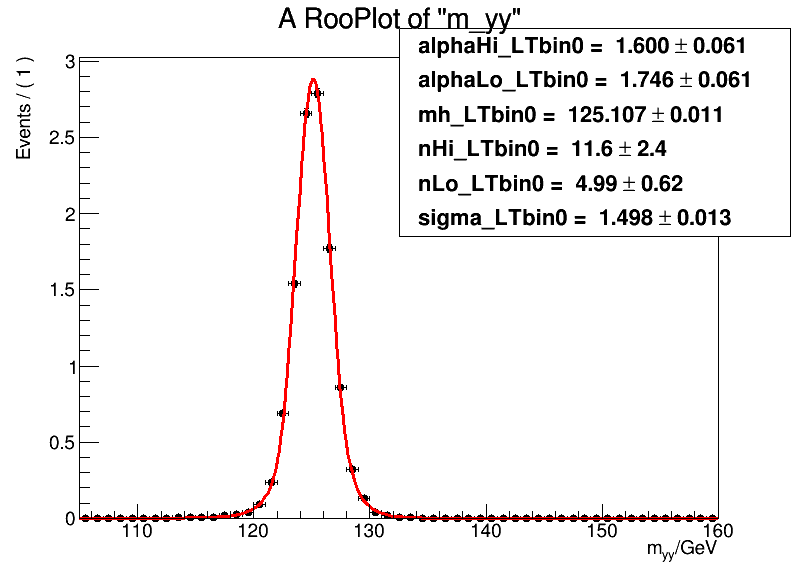
\includegraphics[width=.24\textwidth]{figure/sigmodel/SigFit_LTbin0.png}
  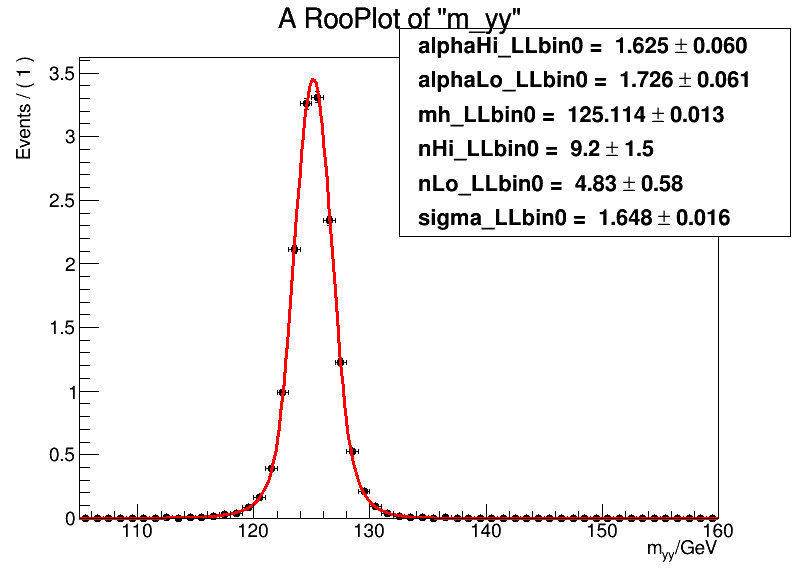
\includegraphics[width=.24\textwidth]{figure/sigmodel/SigFit_LLbin0.png}\\
  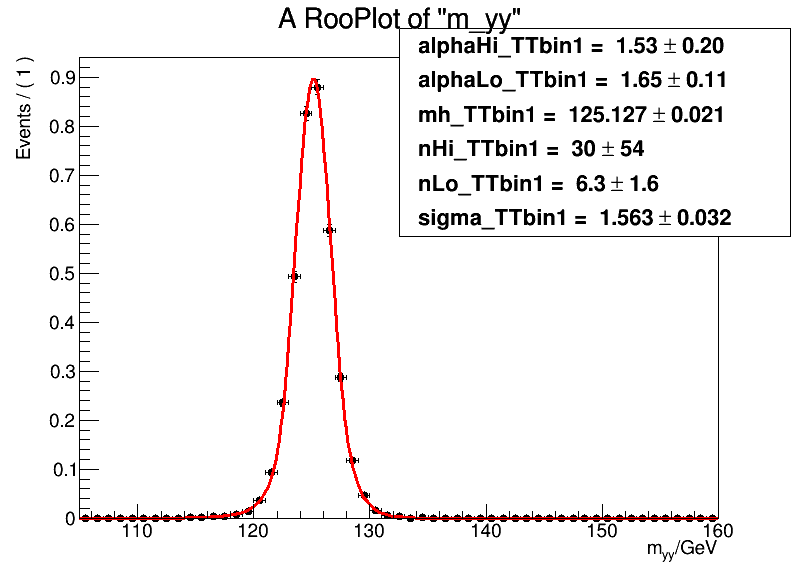
\includegraphics[width=.24\textwidth]{figure/sigmodel/SigFit_TTbin1.png}
  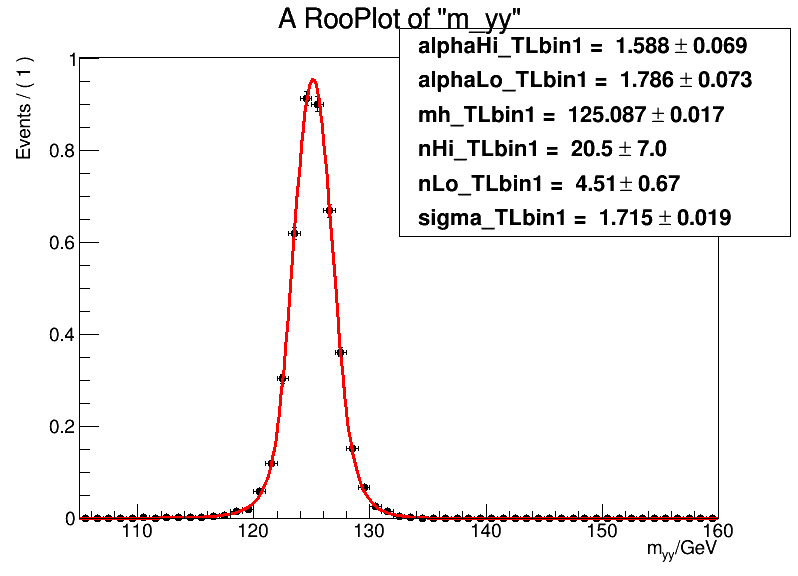
\includegraphics[width=.24\textwidth]{figure/sigmodel/SigFit_TLbin1.png}
  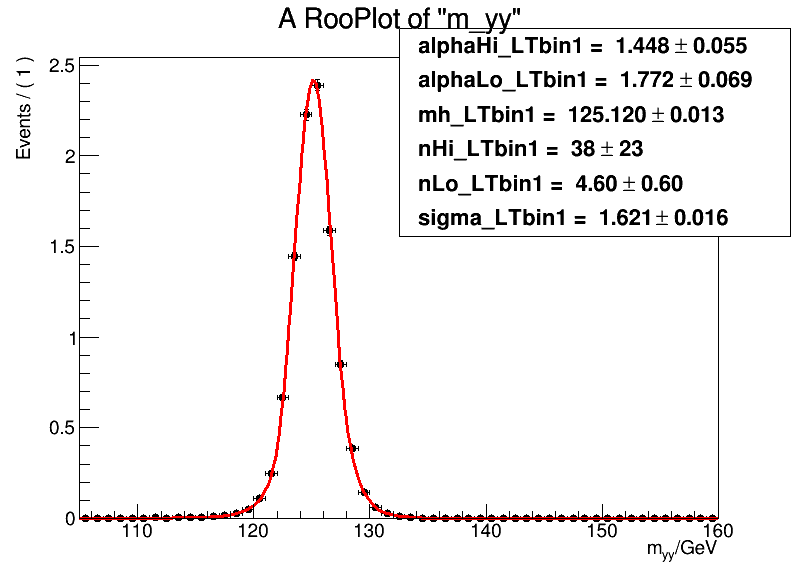
\includegraphics[width=.24\textwidth]{figure/sigmodel/SigFit_LTbin1.png}
  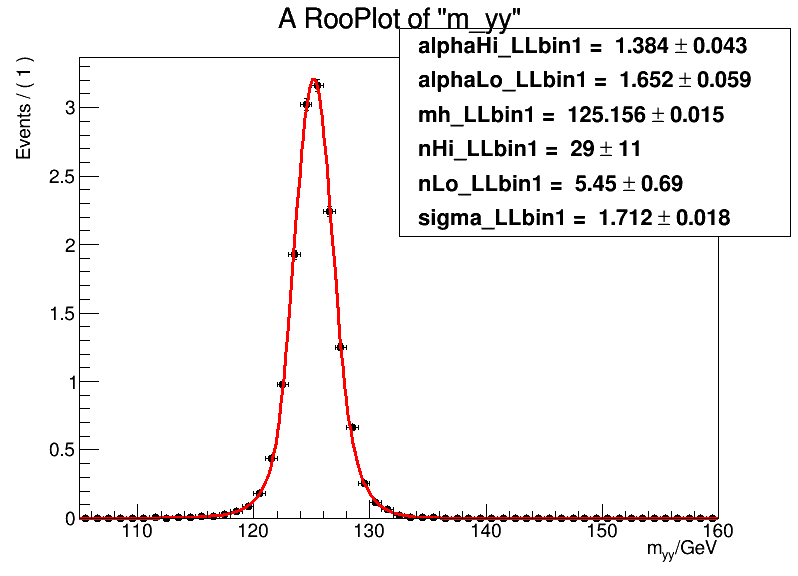
\includegraphics[width=.24\textwidth]{figure/sigmodel/SigFit_LLbin1.png}\\
  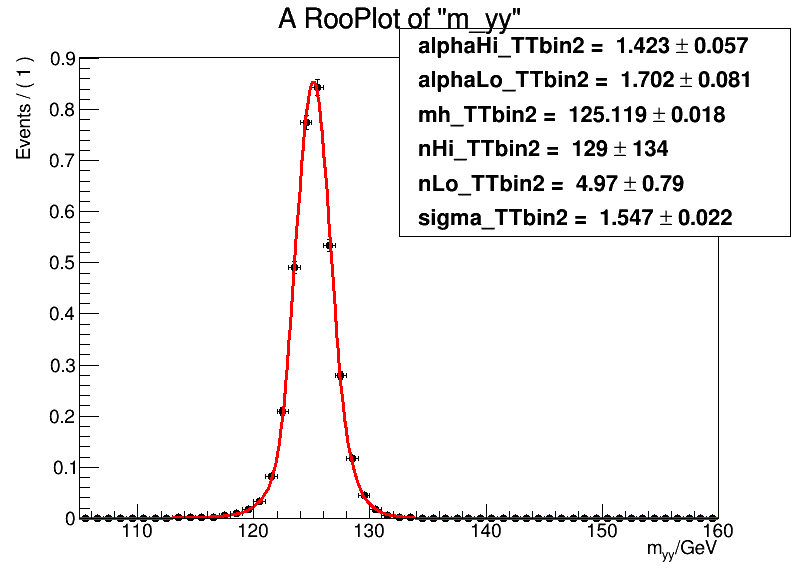
\includegraphics[width=.24\textwidth]{figure/sigmodel/SigFit_TTbin2.png}
  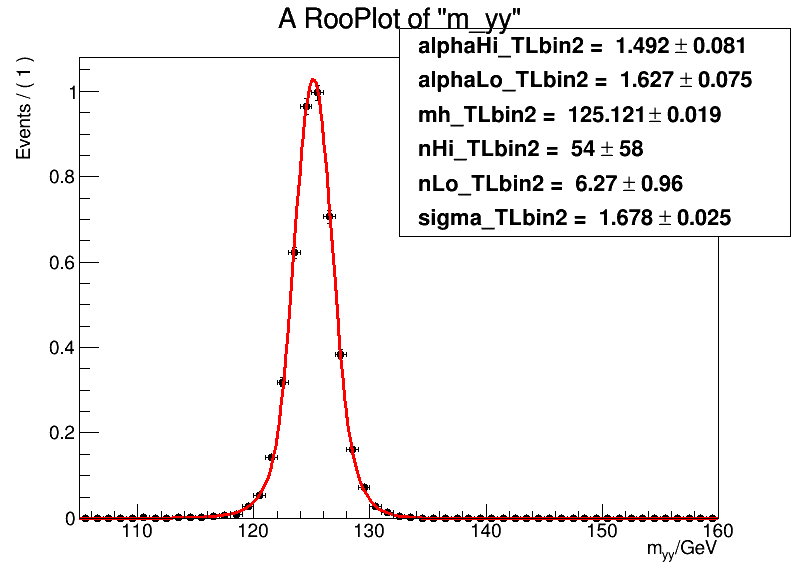
\includegraphics[width=.24\textwidth]{figure/sigmodel/SigFit_TLbin2.png}
  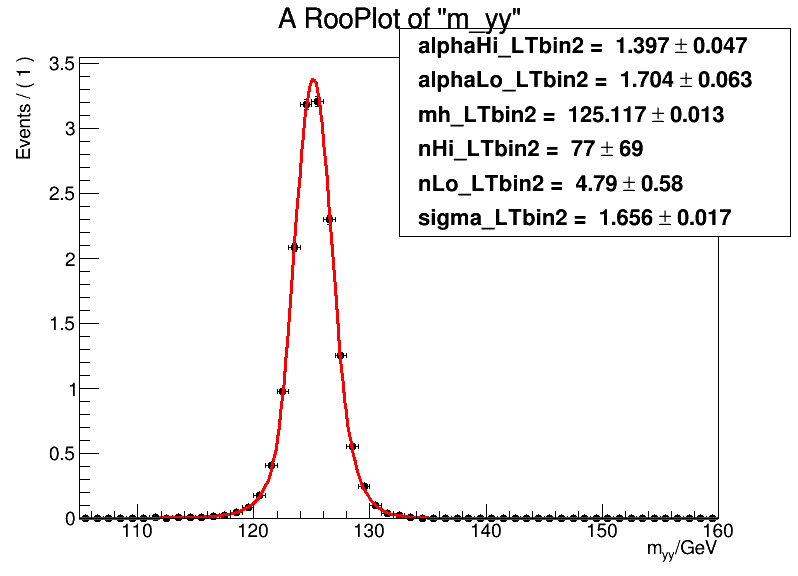
\includegraphics[width=.24\textwidth]{figure/sigmodel/SigFit_LTbin2.png}
  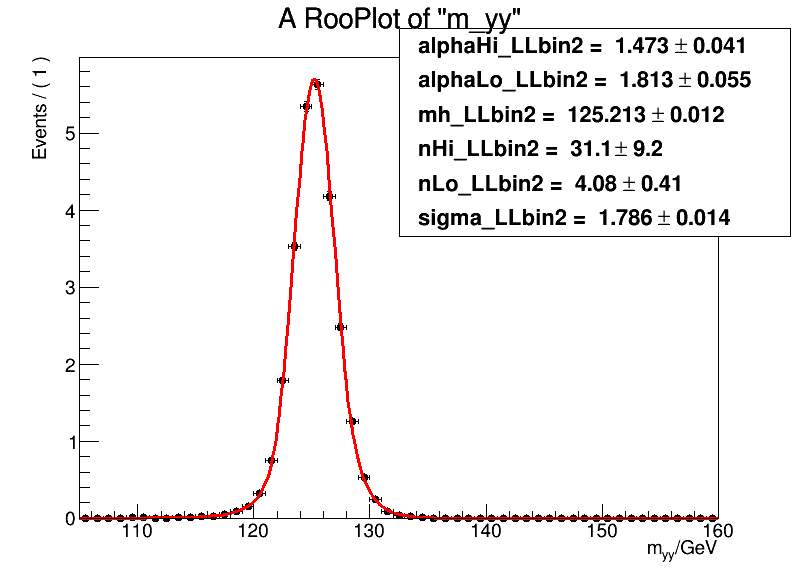
\includegraphics[width=.24\textwidth]{figure/sigmodel/SigFit_LLbin2.png}\\
  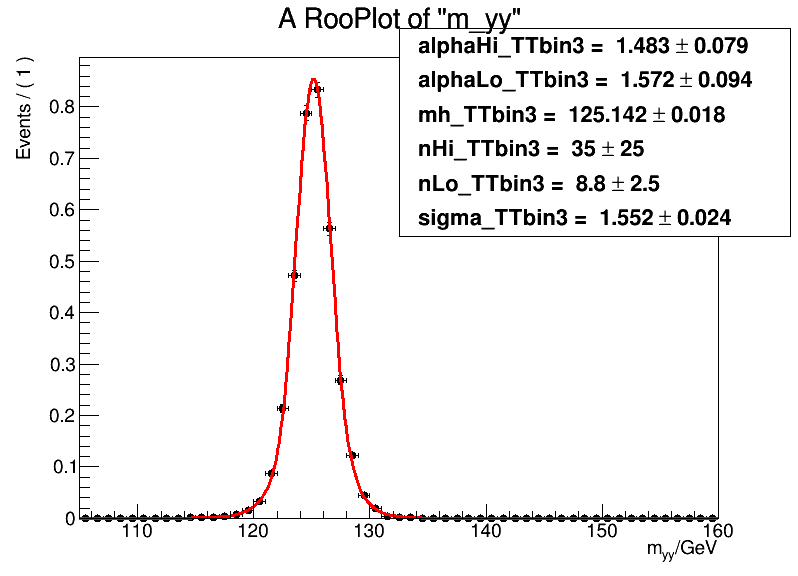
\includegraphics[width=.24\textwidth]{figure/sigmodel/SigFit_TTbin3.png}
  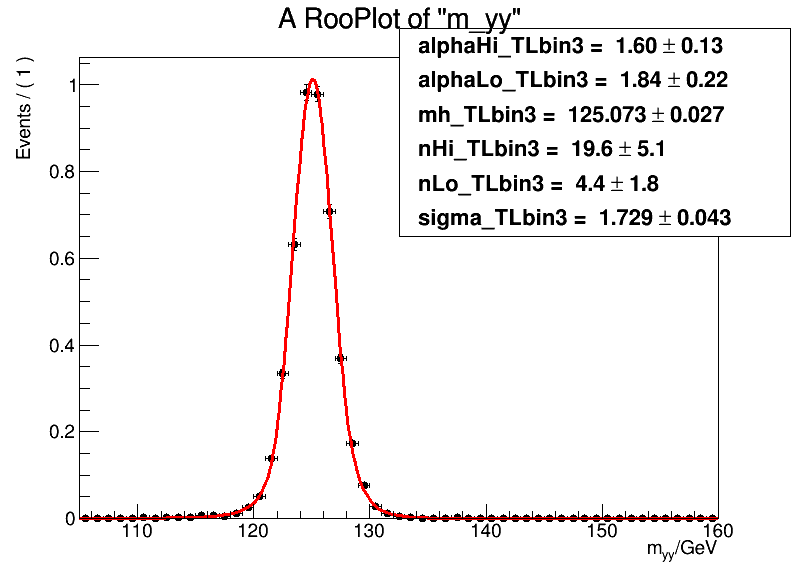
\includegraphics[width=.24\textwidth]{figure/sigmodel/SigFit_TLbin3.png}
  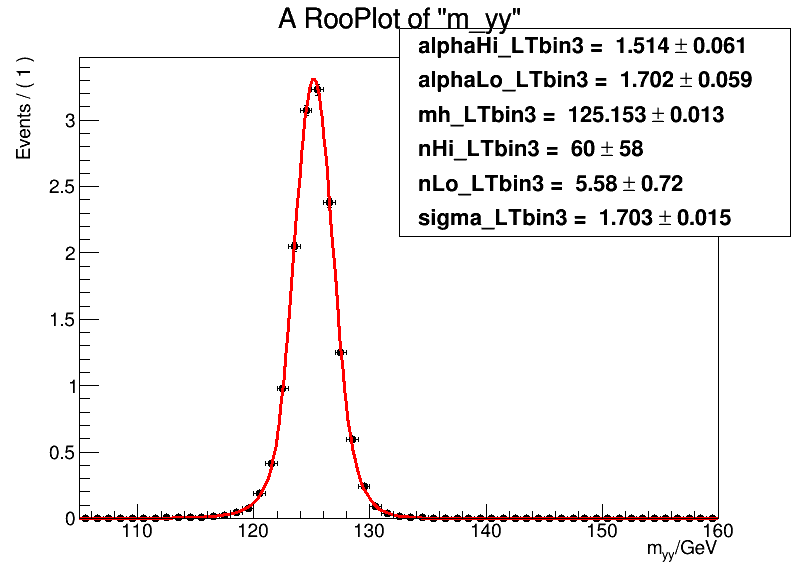
\includegraphics[width=.24\textwidth]{figure/sigmodel/SigFit_LTbin3.png}
  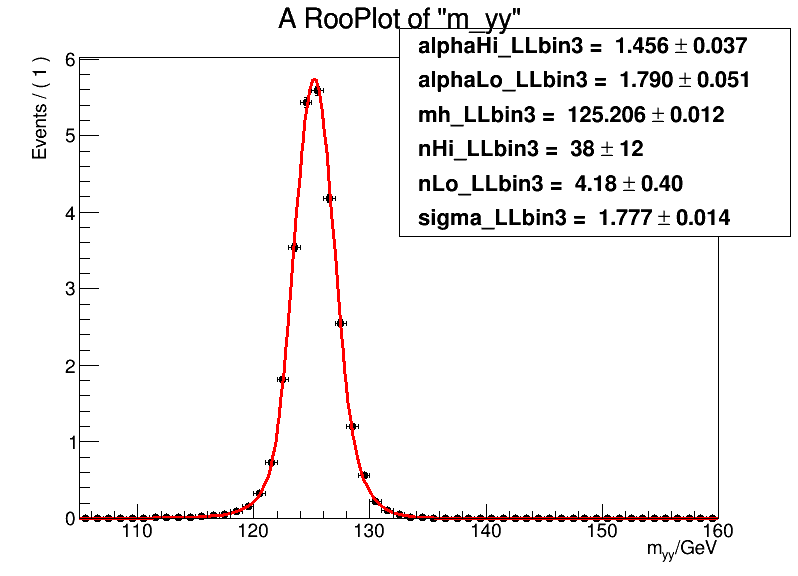
\includegraphics[width=.24\textwidth]{figure/sigmodel/SigFit_LLbin3.png}\\
  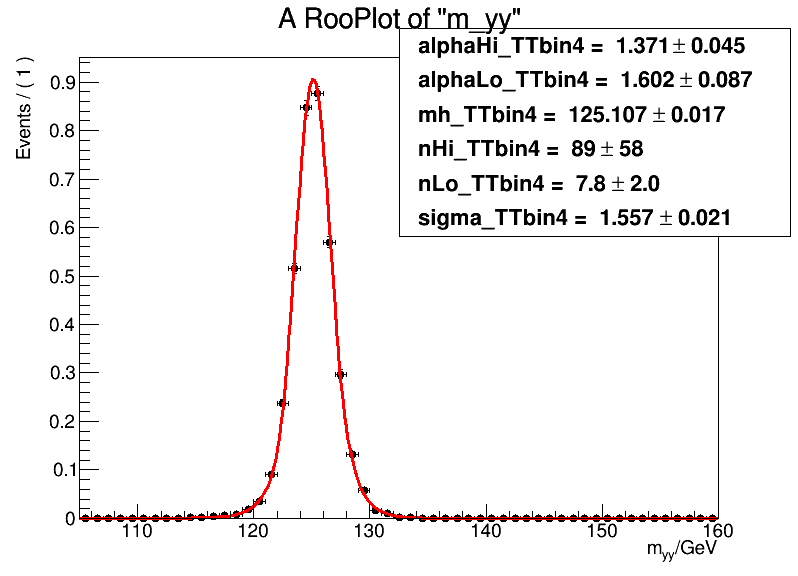
\includegraphics[width=.24\textwidth]{figure/sigmodel/SigFit_TTbin4.png}
  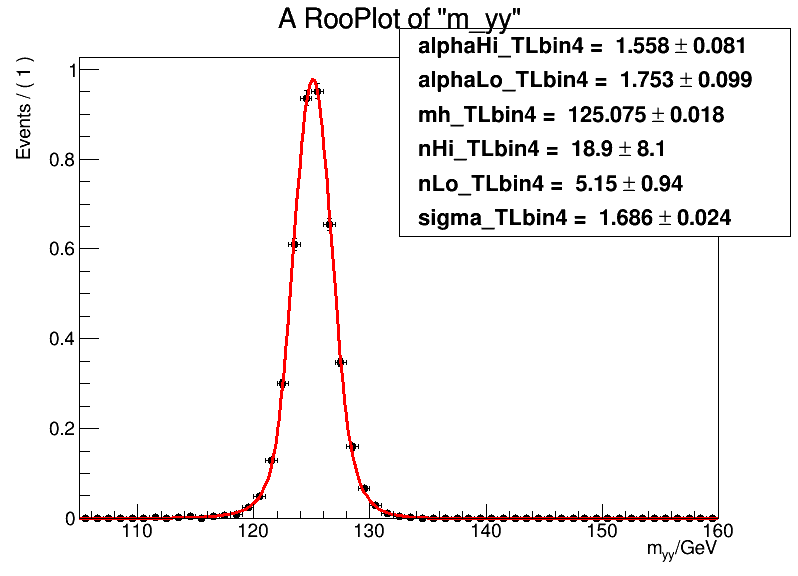
\includegraphics[width=.24\textwidth]{figure/sigmodel/SigFit_TLbin4.png}
  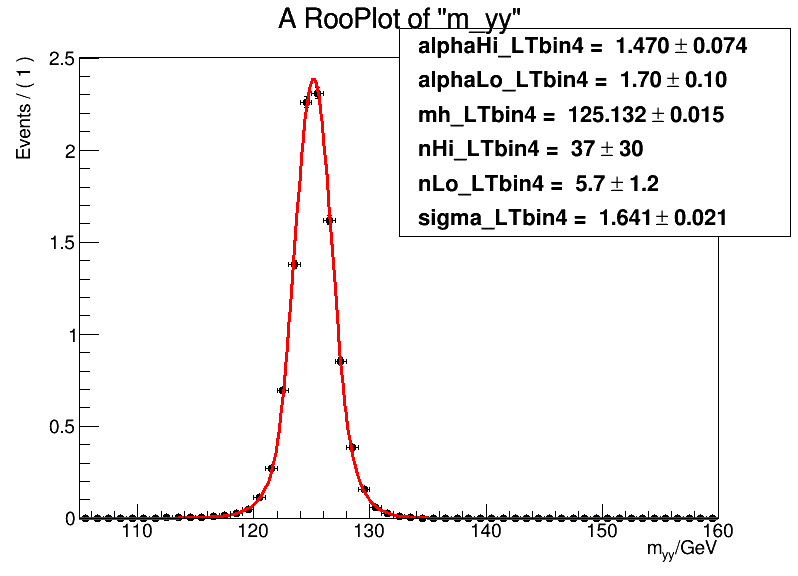
\includegraphics[width=.24\textwidth]{figure/sigmodel/SigFit_LTbin4.png}
  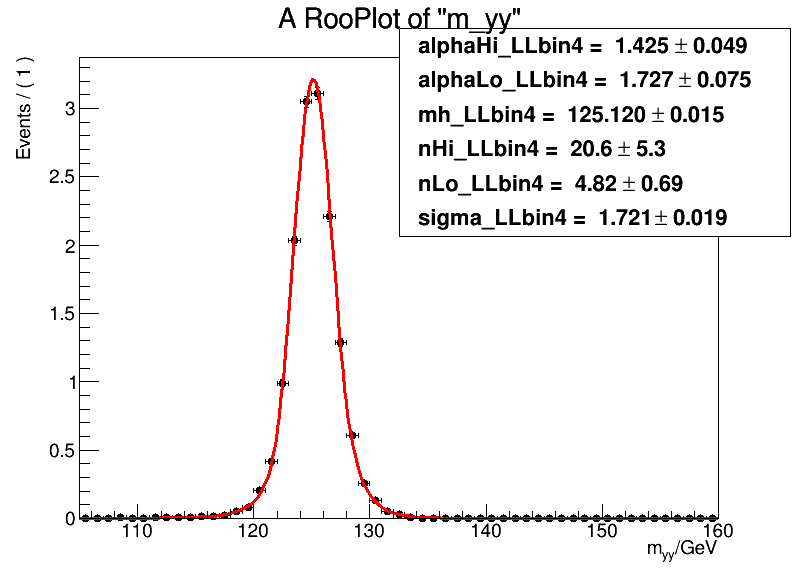
\includegraphics[width=.24\textwidth]{figure/sigmodel/SigFit_LLbin4.png}\\
  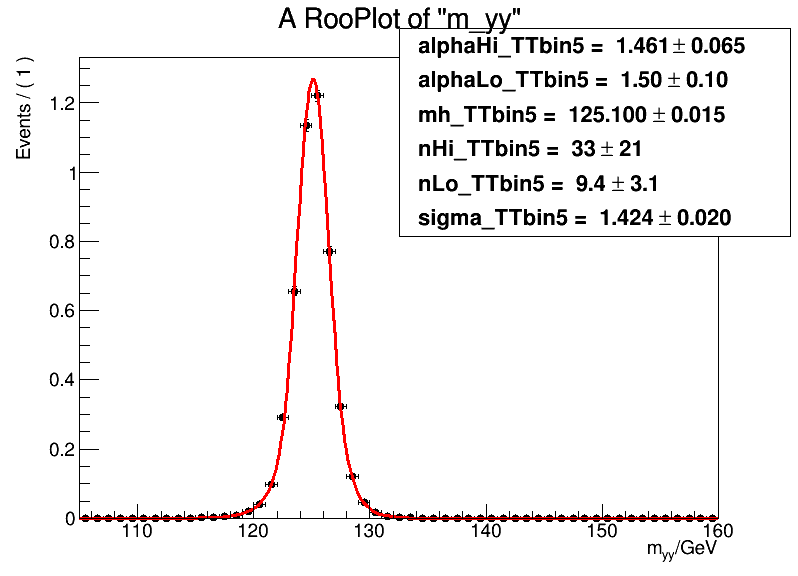
\includegraphics[width=.24\textwidth]{figure/sigmodel/SigFit_TTbin5.png}
  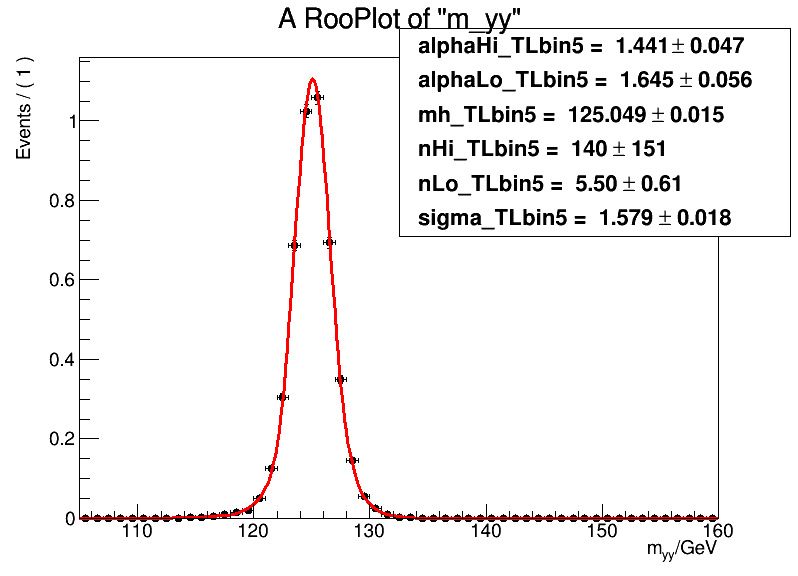
\includegraphics[width=.24\textwidth]{figure/sigmodel/SigFit_TLbin5.png}
  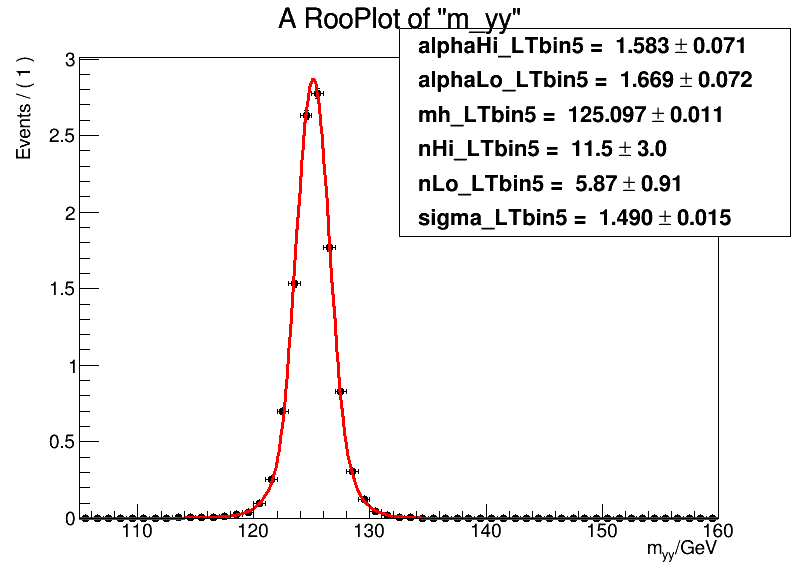
\includegraphics[width=.24\textwidth]{figure/sigmodel/SigFit_LTbin5.png}
  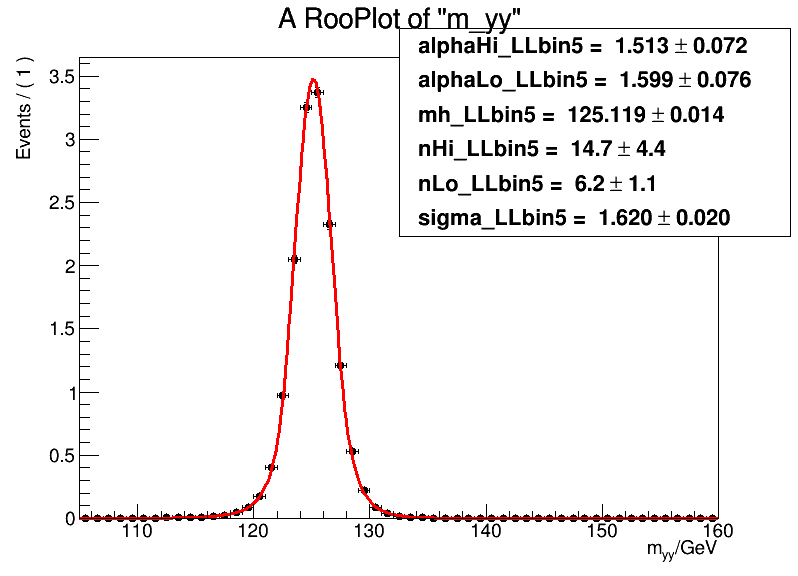
\includegraphics[width=.24\textwidth]{figure/sigmodel/SigFit_LLbin5.png}\\
  \caption{Fitted Doubles Sided Crystal ball shapes for all the reconstructed categories of the analysis. }
  \label{fig:signal_shapes}
\end{figure}

In the final statistical workspace:
\begin{itemize}
	\item the value of \mH is constrained to the one of \RunOne measurement, taking into account its error;
	\item all the six parameters of the DSCB are kept fix during the fit
	\item $\mu_\text{CB}$ and $\sigma_\text{CB}$ are each multiplied by a response function to take into account photon energy scale and photon energy resolution systematics, respectively (see \Sect{\ref{sssec:signal_shape_syst}})
\end{itemize}

